移动之后,移动的对象既没有部分销毁,也没有完全销毁。析构函数还未调用,直到已移动对象的生命周期结束时才调用。因此,析构函数至少要没问题。\par

然而,C++标准库为可移动类型提供了更多的保证。已移动对象处于“有效但未定义的状态”,所以可以像使用任何不知道其值的类型的对象一样使用已移动对象。像使用该类型的非const引用形参,而不知道所传递对象的值一样。例如,我们可以做的不仅仅是销毁已移动对象,还可以使用移动语义来实现排序和可变序列算法。\par

为了更详细地理解如何处理已移动对象,最好区分与之相关的两个信息:\par

\begin{itemize}
	\item C++标准库安全地使用已移动对象的要求是什么?
	\item 应该给已移动对象什么样的保证,才能让这些类型的用户知道如何使用它们?
\end{itemize}

这里至少应该满足C++标准库的要求。\par

\hspace*{\fill} \par %插入空行
\textbf{6.1.1 已移动对象要求的状态}

C++标准库中已移动对象的要求没有什么特别之处。也就是说,对于任何函数,为传递的类型和对象制定的需求也适用于任何内部传递或是移动而来的对象。\par

基本上,必须能够销毁已移动对象。此外,在许多函数中,必须能够将新值赋给已移动对象。\par

例如,考虑如何交换两个对象a和b的值(这可能是排序操作的一部分)。交换的实现通常如下(见图6.1):\par

\begin{itemize}
	\item 将a移动到一个新的临时对象tmp(这样a就变成了一个已移动的对象)。
	\item 将b移动赋值给a(这样b就成为了一个已移动你对象)。
	\item 将tmp移动赋值给b(这样tmp就成了一个已移动对象)。
	\item 销毁已移动对象tmp。
\end{itemize}

\begin{center}
	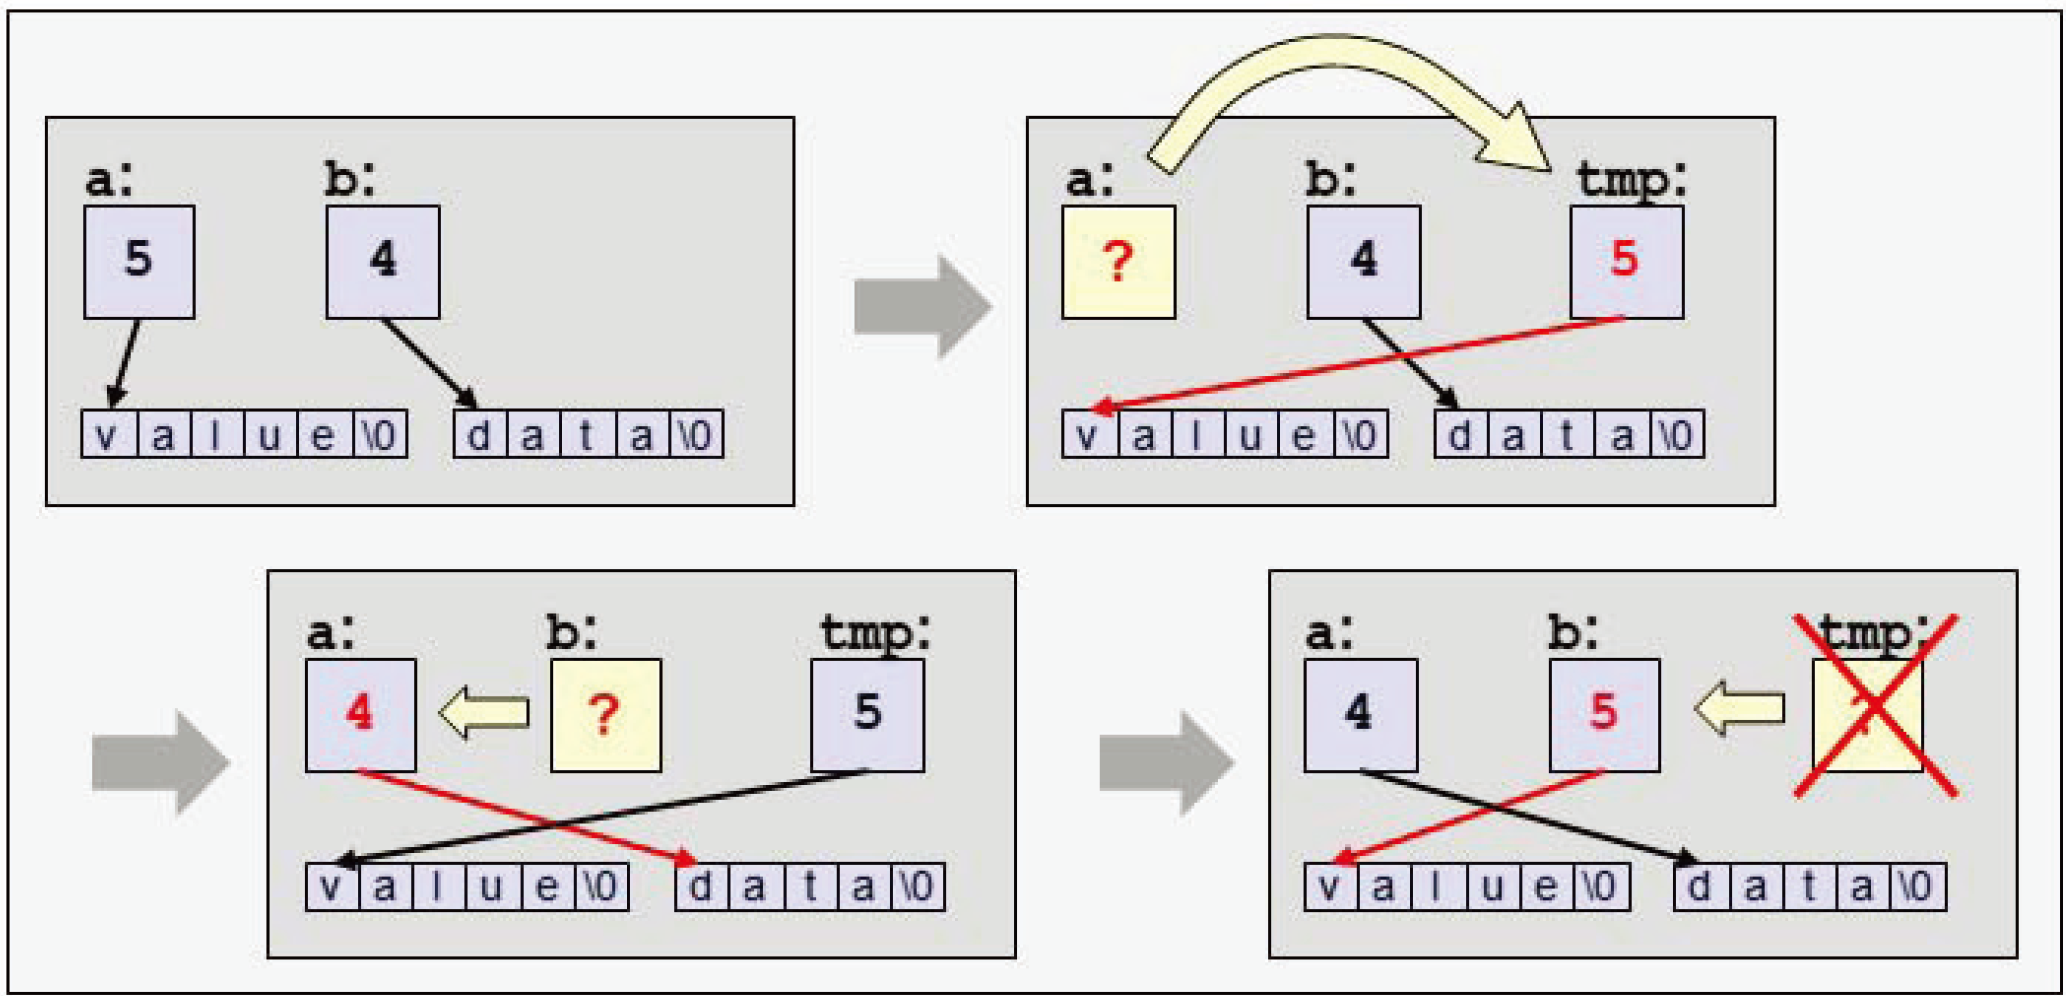
\includegraphics[width=1.0\textwidth]{content/1/chapter6/images/1}
\end{center}

注意,也可以通过向两个参数传递相同的对象来实现自交换。这种情况下,甚至可以将状态为已移动的对象赋值给它自己。\par

所以,对于已移动对象,我们有同样的要求,通常适用于所有对象:\par

\begin{itemize}
	\item 必须能够销毁已移动对象。
	\item 必须能够为m已移动对象赋值。
	\item 应该能够复制、移动或将一个已移动对象赋值给另一个对象。
\end{itemize}

已移动对象还能够处理特殊操作的额外需求。例如,对对象进行排序,所以必须支持<操作或有相应的排序标准。这也适用于已移动的对象。您可能会争辩说,在排序算法中应该知道哪个对象被移动了,这样就可以避免比较它,但C++标准库并不要求这样做。顺便说一下,这也意味着您可以传递已移动对象,对它们进行排序,只要它们支持所有必需的操作就可以了。\par

注意,C++标准库的定义需要的不仅仅是Alexander Stepanov和Paul McJones在《编程元素》一书中所说的部分形成的内容。\par

对于C++标准库中使用的所有对象和类型,应该确保已移动对象也支持所调用函数的所有要求。\par

\hspace*{\fill} \par %插入空行
\textbf{6.1.2 保证已移动对象的状态}

已移动对象的保证定义在使用哪些代码。通常,类的设计者决定给出哪些保证,并且我们总在生命周期结束时销毁对象。对于移动状态,必须提定义良好的析构函数。\par

通常,会有更多要保障的。对于C++标准库的要求,支持基本操作,如复制、赋值相同类型的对象通常就足够了。然而,用户通常希望您还可以处理所有其他方式来为对象赋值。因此,保证可以将一个新值“赋值”给已移动对象就非常有用。\par

考虑给标准字符串s赋新值的不同方法:\par

\begin{lstlisting}[caption={}]
s = "hello"; // assign ”hello”
s.assign(s2); // assign the state of s2
s.clear(); // assign the empty state
std::cin >> s; // assign the next word from standard input
std::getline(myfile, s); // assign the next line from a file
\end{lstlisting}

例如,下面的循环是将流逐行读入vector对象的常见方法:\par

\begin{lstlisting}[caption={}]
std::string row;
while (std::getline(myStream, row)) {
	coll.push_back(std::move(row)); // move the line into the vector
}
\end{lstlisting}

作为另一个例子,可以在处理容器的泛型代码中实现以下语句:\par

\begin{lstlisting}[caption={}]
foo(std::move(obj)); // pass obj to foo()
obj.clear(); // ensure the object is empty afterwards
\end{lstlisting}

类似的代码可以用于释放指针所使用的对象的内存:\par

\begin{lstlisting}[caption={}]
draw(std::move(up)); // the unique pointer might or might not give up ownership
up.reset(); // ensure we give up ownership and release any resource
\end{lstlisting}

通过声明,已移动对象处于有效但未定义的状态,C++标准为其库中的操作进行了保证。\par

例如,以下是根据C++标准定义的行为:\par

\begin{lstlisting}[caption={}]
std::stack<int> stk;
...
foo(std::move(stk)); // stk gets unspecified state
stk.push(42);
... // do something else without using stk
int i = stk.top();
assert(i == 42); // should never fail
\end{lstlisting}

虽然不知道通过\textit{std::move()}将stk传递给foo()后它的值,但只要我们使用它来保存42,直到再次需要它,就可以将它当做一个有效的堆栈。\par

当然,您所提供的保证能达到什么程度取决于您,但是要确保您的类型的用户知道这些保证。通常,他们希望您的类型提供与C++库相同的保证,这样就可以像使用该类型的任何其他对象一样使用已移动对象了。\par

\hspace*{\fill} \par %插入空行
\textbf{6.1.3 破坏不变量}

C++标准库定义了所有处于“有效但未定义状态”的移动对象的含义如下:\par

\textit{对象的值没有指定,除非满足了对象的不变量,并且对象上的操作按照指定的类型进行}\par

不变量是适用于所有可以创建的对象。有了这个保证,可以假定一个从移动的对象处于一种状态,这意味着它的不变量没有破坏。可以像使用非const引用参数一样使用对象,而不知道传递的参数的任何信息:可以调用任何没有约束或前置条件的操作,并且效果/结果是为该类型的其他对象指定。\par

例如,对于一个已移动的字符串,我们可以执行所有没有先决条件的操作:\par

\begin{itemize}
	\item 查询大小
	\item 打印出来
	\item 遍历字符
	\item 转换为C字符串
	\item 分配新值
	\item 添加字符
\end{itemize}

此外,所有这些函数具有语义:\par

\begin{itemize}
	\item 返回的大小可用于安全地调用索引操作符。
	\item 返回的大小与迭代时的字符数相匹配。
	\item 遍历字符时,打印的字符与字符序列匹配。
	\item 添加一个字符将把该字符放在值的末尾(不知道是否还有其他字符在前面)。
\end{itemize}

开发者可以利用这些保证(参见上面的std::stack<>的例子)。\par

有时候,您必须明确地确保不破坏不变量。默认的特殊移动成员函数可能无法正常工作。我们将在下面的小节中讨论示例。\par

\hspace*{\fill} \par %插入空行
\textbf{受限的不变量}

不把c++标准库的全部保证给已移动状态也可以。也就是说,您可能有意地限制已移动对象的可能操作。例如,当一个对象的有效状态总是需要诸如内存之类的资源时,只有一个部分支持的状态可能会更好地降低移动操作的成本。\par

不把C++标准库的全部保证给已移动状态也是有用的。也就是说,可能要有意地限制已移动对象的可能操作。例如,当一个对象的有效状态总是需要内存之类的资源时,只支持一个部分的状态可能会更好地降低移动操作的成本。\par

理想情况下,不支持所有操作的状态应该是可查的。对象应该知道这个状态,并提供一个成员函数来检查这个状态。已移动对象也可能拒绝执行此状态下不支持的操作。然而,在一般情况下,相应的检查可能会影响性能。\par

在C++标准库中,有些类型提供了API来检查对象是否处于移出状态。例如,std::futures有一个成员函数valid(),该函数对已移动对象返回false。所以,不同对象检查状态是否移动的接口不同。\par

通常,已移动状态是默认构造状态,这意味着已移动状态无论如何都是不变量的一部分。在任何情况下,需要让用户知道什么是可用的,什么不可用。\par




